\documentclass{my_cv}
\usepackage{titlesec}
\usepackage{graphicx}
\usepackage{hyperref}
\begin{document}
	\name{Anuj Trehan}
	
	\begin{center}
		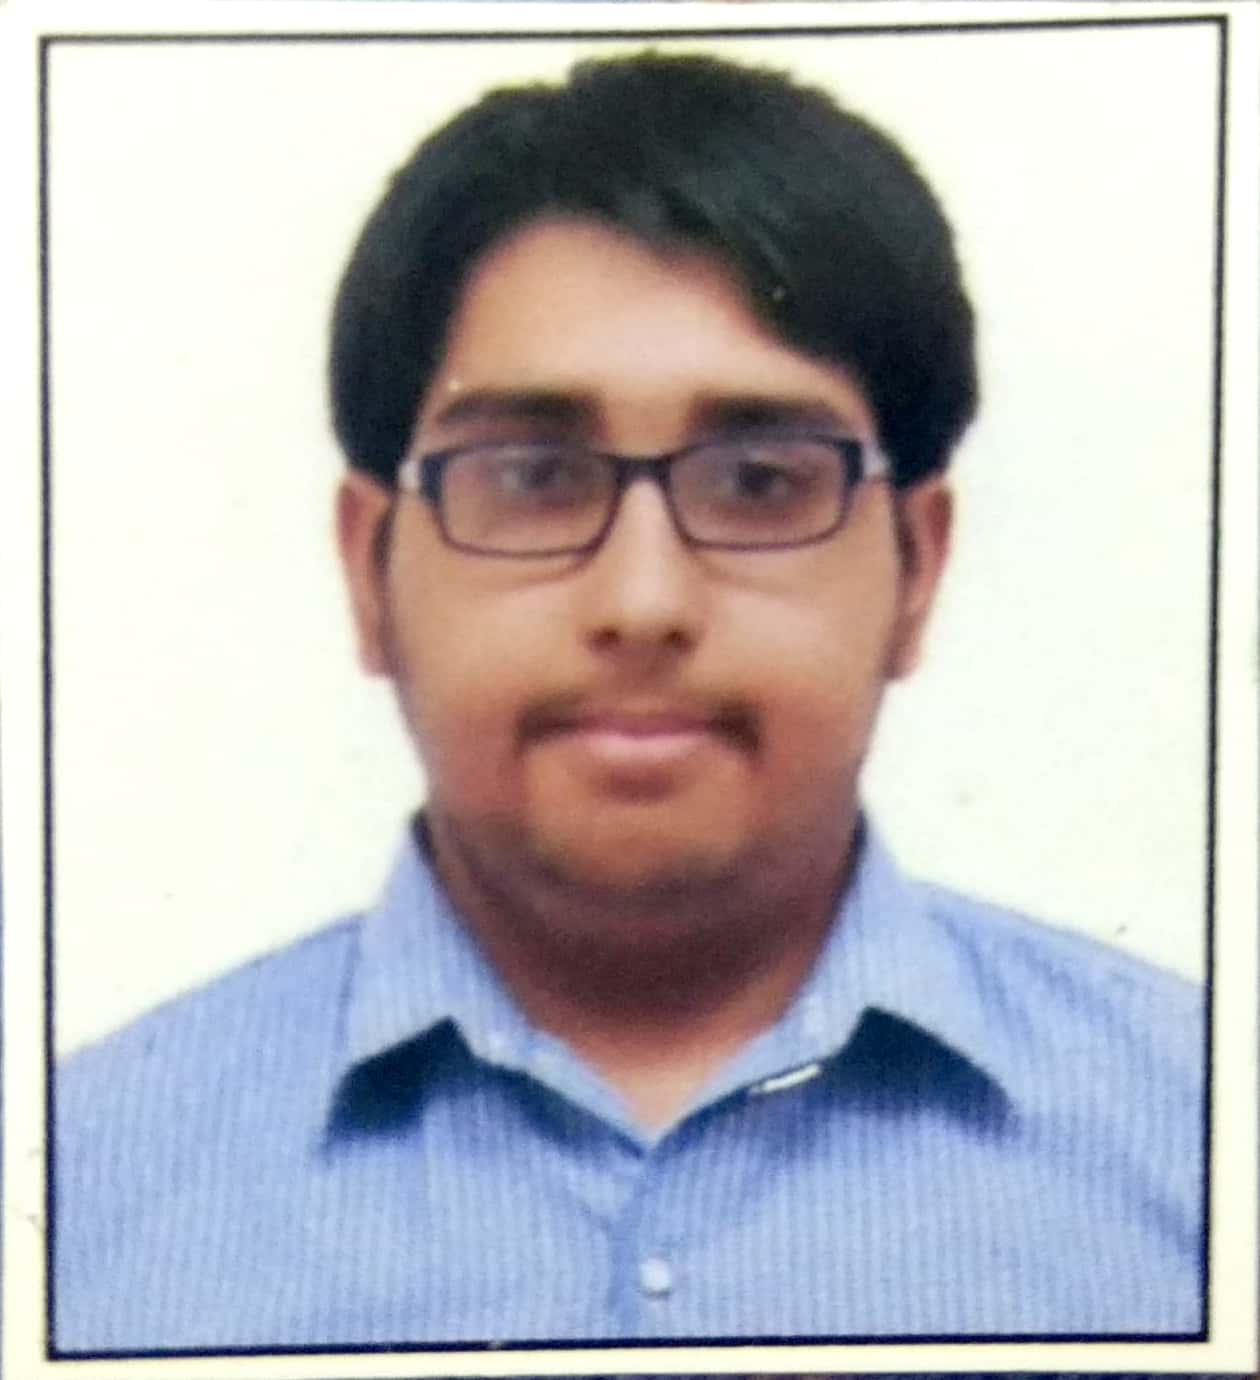
\includegraphics[width=3cm, height=3cm]{Anuj.jpg}\\
	\end{center}
	
	\contact{C-45 New Krishna Park,Vikas Puri}{New Delhi-18}{atrehan789@gmail.com}{+91 9999616069}
	
	\section{Career Objective}
	
	
	The main goal of my career is to help people using Artificial Intelligence and Internet as in my opinion if these two can be combined and used correctly we can create wonders.Also I believe in the power of education and have a vision to empower everyone with right type of education.
	
	\section{Education}
	
	\begin{tabular}{|l|l|l|l|l|}
		\hline
		Deg./Sem & Institute & University/Board & Passing year & Perc/CGPA \\
		\hline
		Semester 2 & B.V.C.O.E. & G.G.S.I.P.U. & 2018 & 9 \\
		\hline
		Semester 1 & B.V.C.O.E. & G.G.S.I.P.U. & 2017-18 & 9 \\
		\hline
		AISSCE & St. Cecilia\'s Public School & CBSE & 2017 & 92.4\%  \\
		\hline
		
		10$^{th}$ Board & St\. Cecilia\'s Public School & CBSE & 2015 & 9.4  \\
		\hline
	\end{tabular}
	\section{Projects}
	  \begin{enumerate}
	  	\item \href{https://github.com/anuj2110/lstm-music-gen}{Music Generation With Deep Learning:An LSTM based Seq2Seq neural network which is trained to predict the next note in a music played with piano.}
	  	
	  	\item \href{https://github.com/anuj2110/keras}{Image Generation With Deep Learning:Vaious types of Autoencoders were used to generate images of some given kind.Includes normal and Convolutional Autoencoders.}
	  	\item \href{https://github.com/anuj2110/LaneDetection}{ Lane Detection With Computer Vision:
	  		An Pipeline was genrated wherein a video of a road is given and the lane lines are marked on the video where there are lanes.}
	  	\item \href{https://github.com/anuj2110/neural-style-transfer}{Neural Style Transfer:A Convolutional Neural Network based approach wherein two images are given and the style of one image was overlayed on the other.}
	  	\item Facial Expression Recognition With Deep Learning:
	  	A Convolutional Neural Network was used to identify 7 different human Expressions based on the images of their faces used as input.
	  	\item Playing Games With Deep Learning: A Deep Neural Network was trained to Play a game in openAI gym environment Lunar Lander.
	  \end{enumerate}
	\section{Training and Internships}
		\begin{itemize}
			\item Attended Innovicon (AI conference Held at B.V.C.O.E.): 2-3 February 2019.
			\item Attended Google MLCC ( at B.V.C.O.E.): October 2018.
			\item Attended Actions On Google Workshop series (at B.V.C.O.E.): July 2018.
			\item Attended Deep Learning Workshops (at B.V.C.O.E.): March-April 2018.
			\item Took the Convolutional Neural Networks Course offered by deeplearning.ai at Coursera platform.
			\item Attended Machine Learning Workshops organised by DSC in B.V.C.O.E: March 2018
			 
		\end{itemize}
	\section{Research Publication}
	\begin{enumerate}
		\item Null
	\end{enumerate}
	\section{Technical Skills}
	\begin{itemize}
		\item Languages Known: C++,Python
		\item Opensource Libraries used: Numpy,OpenCV,Tensorflow/Keras,PyTorch,Flask
		\item Operating Systems Worked upon : Windows and Ubuntu
		\item Version Control Systems used Git
	\end{itemize}
	
	\section{Soft Skills}
	\begin{enumerate}
		\item Event Management
		\item Public Speaking
		\item Tecnical Writing(Started a Blog Post for IEEE(SIG OF B.V.C.O.E.))
	\end{enumerate}
	
	\section{Extra Curricular Activites}
		\begin{itemize}
			\item Volunteering at NSS B.V.C.O.E.
			\item Volunteering at BVPIEEE
			\item Volunteered in hosting a competition "Plan For India"
			\item TechieBytes Medium Page for BVPIEEE
		\end{itemize}
	\section{Co-Curricular Activites}
		\begin{enumerate}
			\item Graphic Designing (Mainly posters and Logos)
		\end{enumerate}
	
	
    \section{Personal Details}
 
 	\begin{tabular}{ll}
    	\textsc{Father's Name:} & Harish Trehan \\
    	\textsc{Mother's Name:}       & Bhawna Trehan \\
    	\textsc{Gender:}         & Male \\
    	\textsc{Date Of Birth:}         & 21 October 1998 \\
    	\textsc{Nationality:}   & Indian \\
    	\textsc{Marital Status:} & Single \\
    \end{tabular}
	\section{Declaration}
	I here by Declare that the information provided by me is true to the best of my knowledge.
	
	

\end{document}
 